\chapter{PROGRAMMING MACROS}

\addtocimage{-10pt}{-40pt}{../graphics/harnett.jpg}

\pagebreak
\setlength\columnsep{1.5em}

\thispagestyle{plain}
\pagestyle{headings}
{\centering  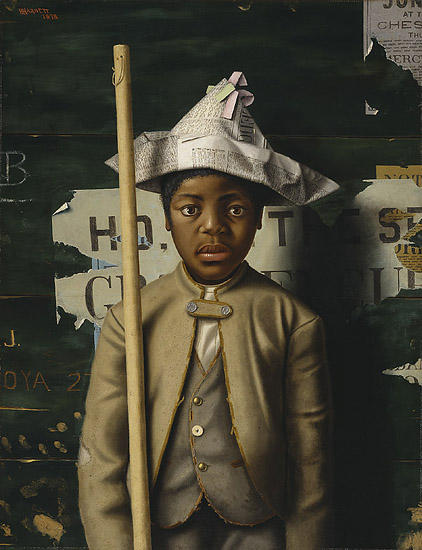
\includegraphics[width=0.7\linewidth]{./graphics/harnett.jpg}\par}

\newcommand*{\newacronym}[1]{{New acronym: [#1]\par}}
\newcommand*{\newacronyms}{%
  \let\do\newacronym
  \docsvlist
}
\vspace{1.5\baselineskip}
{\centering \Large\bf GETTING STARTED WITH MACROS\par}
\bigskip

\begin{multicols}{2}
\lettrine{P}{rogramming} with \alltex is done through macros. \tex has a macro programming language,
which allows features to be added. The best known
and most widely used collection of \tex macros is \latex.
(This is not quite accurate. Although originally
\latex used \tex, since 2003 it by default uses
e-TEX, which is an extension of TEX. Macro's in \TeX\  are not just simple substitutions, they are more Lispy like. It is this powerful feature that made \TeX\ last and will continue to do so for many years to come. This program that started as a typesetting program, programmed in a variant of what is now an ancient computer language Pascal is testimony to good programming 
practices and a reminder to the programming priesthood that the tool is not important, but what you do with it is. 

A \emph{macro} is a sequence of tokens that has been abbreviated into a control sequence. Statement starting with among others
\cmd{def} are called \textit{macro definitions}. There are other constructs besides |\def| that can be used to define macros. \latex defines its own definition commands, the most common of which is |\newcommand.| The way \tex's macro language is build, you can also define your own. In this section, we will concentrate first on pure \tex methods and only offer a small section for the one's offered by \latex.

\end{multicols}
\clearpage

\section{How to define macros}

Most of \tex programming is learning how to work with macros and control sequences. The workhorse behind all these is a three letter control sequence that can be used to define macros \refCom{def}.
There are other macro defining primitives available, but we will first focus on \refCom{def}. Depending on the way the arguments of the command are specified these are normally divided into two general categories: \emph{delimited macros} and \emph{undelimited}.
 
\subsection{Simple substitution macros}

\begin{docCommand*}{def} { \meta{macro name}\meta{parameter text}} {\marg{replacement text}}
Simple substitution macros, during expansion replace their name with the contents enclosed between the braces. For example some common macros that authors write, is to hold the names of people, in order to get the spelling correctly.
\end{docCommand*}

\begin{teX}
\documentclass{article}
\def\myshortcut{Anthony van der Merwe}
\begin{document}
\myshortcut
\end{document}
\end{teX}


In the above we defined a macro named, |\myshortcut|, will print the name \texttt{Anthony van der Merwe}, every time it is invoked as |\myshortcut|. You will notice, that the macro definition is placed in the preamble. This is not necessary, but it is good practice. Macros can be placed anywhere in the document, in packages and or classes.


If we were writing the macro and compiling it using \tex only, the example can be much shorter and it will also compile much faster. 

\emphasis{def}
\begin{teX}
\def\myshortcut{Anthony van der Merwe}
\myshortcut
\bye
\end{teX}

Macros can use other macro commands. For example if we wanted to store the name of the author of |pdfTeX| we could write,

\begin{texexample}{example substitution macro}{}
\def\Thanh{%
      H\`an~%
      \texorpdfstring{Th\^e\llap{\raise 0.5ex\hbox{\'{}}}}%
      {\ifpdfstringunicode{Th\unichar{"1EC3}}{Th\^e}}%
      ~Th\`anh^^a
    }
\Thanh 
\end{texexample}




\subsection{Macro parameters.} 

In this Chapter we will spend most of the time with commands available in \tex core, before we move onto commands that are available in \latex. Now, in the example above, we did not use any parameters. \tex allows us to define parameter by adding |#1|..|#9| as parameters to the macro definition. Here is a short example, again using plain \tex. 


\begin{teX}
\def\twonumbers#1#2{(#1,#2)} 
\twonumbers{12,13}
\bye
\end{teX}

\def\twonumbers#1#2{(#1,#2)}
This will print \texttt{\twonumbers{12}{13}}. The macro takes the two arguments 12 and 13  and prints the two numbers in parentheses. This activity is called \textit{macro expansion}\index{macros>expansion}\index{macros>parameters}.

 
\section{Delimited arguments}

As a simple example consider the following:\index{macros>delimited}

\begin{teX}
\def\asentence#1#2;{{\textbf{#1}#2}}
\bye
\end{teX}

\begin{texexample}{delimited examples}{ex:delimited}
\def\asentence#1#2;{#1}
\asentence The whole sentence is printed;
\end{texexample}

Example~\ref{ex:delimited} defines a macro with an undelimited first parameter, and a second parameter delimited by a semicolon. The replacement text consists only of |#1| and hence the rest are discarded.

\begin{texexample}{delimited examples}{ex:delimited}
\def\asentence#1#2;{{\bfseries #1}#2}
\asentence The whole sentence is printed;
\end{texexample}

Example~\ref{ex:delimited} defines a macro with an undelimited first parameter, and a second parameter delimited by a semicolon. The replacement text consists only of |#1| and hence the rest are discarded.


\subsection{Space, return, and the tab character as delimiters of parameters}

A space can be used to delimit a parameter. The space character, return character and the tab character are all converted into space tokens by \tex. Here is an example,

\begin{texexample}{Space delimiters}{ex:spacedelimiters}
\def\tempmacro #1 #2 #3 {#1,#2,#3}
\tempmacro 12 15 17 
\end{texexample}


\section{Format of a macro definition}

So far we have looked at macros that have no parameters, macros that have parameters and macros that have delimited arguments. A macro definition consists of, in sequence,

\begin{enumerate}
\item any number of \cmd{\global}, \cmd{\long}, and \cmd{\outer}, prefixes
\item a \cmd{\def} control sequence, or anything that has been \cmd{\let} to one,
\item possibly a parameter text specifying among other things how many parameters the macro has,
\item a replacement text enclosed in explicit characters \{\}
\end{enumerate}


\CMDI{\global}\cmd{\def}\meta{command}\{\ldots\}

As the name implies global macros define macros that they have a global scope. \TeX, like many other computer languages has scoping rules. We will revisit \tex's scoping rule in the Chapter for Grouping.  Try the following example:


\begin{teX}
\def\sometext{This is some text}
\def\someothertext{%
   \def\sometext{I am in the macro, someothertext.}\par
   \sometext
}
\sometext
\end{teX}

\def\sometext{This is some text}
\def\someothertext{%
   \def\sometext{I am in the macro, someothertext.}\par
   \sometext
}
\sometext
\someothertext

As you can see from the output, any definitions of macros within other macros are defined locally within the scope of the aprent macro only. I am also sure that you have also observed that we can nest macros to as many depths as required.

\def\sometext{This is some text}

\def\someothertext{%
   \gdef\sometext{I am in the macro, someothertext.}\par
   \sometext
}

\sometext

\someothertext

\sometext

\CMDI{\long}\cmd{\def}\marg{command}\{\ldots\}

\index{macro definitions>long}
Knuth designed \tex in such a way that the normal |\def| will not work with arguments that include paragraphs. This was so that if you forget to add a brace '\}' \tex will not continue absorbing tokens until the end of the file or completely full \tex's memory. Therefore \tex has another rule [205] intended to confine errors to the paragraph that they occur: The token |\par| is not allowed to occur as part of an argument as unless you explicitly tell \tex that you want to use |\par|. Whenever \tex is about to include |\par| as part of an argument, it will abort the current macro expansion and report that a \texttt{...runaway argument} has been found.

If you actually want a control sequence to allow arguments with |\par| tokens, you can define it to be a \cmd{\long}\index{macros>long} just before the |\def|. For example the |\bold| macro defined by:


\begin{teX}
\long\def\bold#1{{\bf#1}}
\end{teX}

\noindent is capable of setting several paragraphs in boldface type. However, such a macro is not a especially good way to typeset bold text. It would be better to say, e.g.,

\begin{teX}
\def\beginbold{\begingroup\bf}
\def\endbold{\endgroup}
\end{teX}
because this doesn't fill \tex's memory with a long argument.


\CMDI{\edef}
\index{macro definitions>\string\edef=\texttt{\string\edef}}

Another command that can be used to define macros is \cmd{\edef}. You can say |\edef\foo{bar}|. The syntax is the same as |\def|, but the token list in the body is fully expanded (tokens that come from |\the| are not expanded).

You can say |\xdef\foo{bar}|. The syntax is the same as \cmd{\def}, but the token list in the body is fully expanded (tokens that come from \cmd{\the} or \cmd{\unexpanded} are not expanded).

\CMDI{\global}\cmd{\edef}

You can put the prefix \cmd{\global} before \cmd{\xdef}, this is however useless, since |\xdef| is the same as |\global\edef|. The following example puts a brace in |\foo|. The |\string| command can be expanded, the value is the name of the command (preceded by a backslash, or whatever the value of the escape character is). Here the assignment to the escape character is local, the assignment to |\foo| is global.


\begin{teX}
{\escapechar=-1 \xdef\foo{\string\}}}
\end{teX}


\CMDI{\relax}\quad 

The control sequence \cmd{relax} cannot be expanded, but when it is executed \textit{nothing happens}.
This statement sounds a bit paradoxical, so consider an example. 


\begin{codeexample}[]
\newcount\MyCount
\newcount\MyOtherCount \MyOtherCount=2
\MyCount=1\number\MyOtherCount3\relax4\par

\the\MyCount
\end{codeexample}

\CMDI{\number}

The command \cmd{\number} is expandable, and \cmd{\relax} is not. When TEX constructs the number that is
to be assigned it will expand all commands, either until a non-digit is found, or until an unexpandable
command is encountered. Thus it reads the 1; it expands the sequence \verb+ \number\MyOtherCount+,
which gives 2; it reads the 3; it sees the \cmd{\relax}, and as this is unexpandable it halts. The number
to be assigned is then 123, and the whole call has been expanded.


\noindent Since the \cmd{\relax} token has no effect when it is executed, the result of this line is that 123 is
assigned to \verb+ \MyCount +, and the digit 4 is printed.



Another example of how \cmd{\relax} can be used to indicate the end of a command is

\verb+ \MyCount=123\relax4+

\begin{codeexample}[]
\newcount\MyCount
\MyCount=123\relax4\par
\the\MyCount
\end{codeexample}

\noindent Since the \cmd{relax} token has no effect when it is executed, the result of this line is that 123 is
assigned to \verb+ \MyCount +, and the digit 4 is printed.

Another example of how \cmd{relax} can be used to indicate the end of a command is


\begin{teX}
\everypar{\hskip 0cm plus 1fil }
\indent Later that day, ...
\end{teX}

\noindent This will be misunderstood: TEX will see

\verb+ \hskip 0cm plus 1fil L+

\noindent and fil L is a valid, if bizarre, way of writing fill (see Chapter 36). One remedy is to write

\verb+ \everypar{\hskip 0cm plus 1fil\relax}+

\section{Spaces after macro calls}

\CMDI{\ignorespaces}
The primitive \cmd{\ignorespaces} allows the user to unify the calls of certain macros. Consider the following:

\begin{codeexample}[]
\bgroup
\def\\{A}
\def\xx{..}
\def\yy{...}

\\ABC
\\ ABC
\xx ABC
\yy{1}ABC
\yy{a} ABC
\egroup
\end{codeexample}

As it can be observed from the example spaces after control\textit{symbols} like |\\| are \emph{not ignored}, and therefore the output from line 1 reads ``AABC" and the output from line 2 reads ``X ABC. To bring some uniformity to the treatment of spaces after macro calls (regardless of whether the macro has parameters or not, the \cmd{\ignorespaces} primitive can be used. Including this instruction as the \emph{last} token in the replacement text of a macro causes the space (or any number of space tokens) following the macro call to be ignored.

%\begin{codeexample}[]
\bgroup
\def\\{A\ignorespaces}
\def\yy{...\ignorespaces}

\\ABC
\yy{a}\ignorespaces ABC
\egroup
%\end{codeexample}

Note that \cmd{\ignorespaces} does \emph{not} cause \tex to gobble up empty lines following the macro call because \tex converts empty lines into \cs{par}s. 

\cmd{\ignorespaces} does nothing, if no space token or space tokens follow it.  However, it \emph{does} expand token follow it though to find out whether they contain space tokens or not.

\section{Creating macros on the fly}


One of the more useful ability of \tex is that macros can be created programmatically. This is achieved using \cmd{\string} and \cmd{\csname}

\footnote{Most of this discussion is based on an article by Stephan v. Bechtolsheim see \url{http://www.tug.org/TUGboat/Articles/tb10-2/tb24bechtolsheim.pdf}}

This article discusses \cmd{\string} and \cmd{\csname} to
convert back and forth between strings and tokens.
To control loading macro source files in a convenient
way, I will show an application of \cmd{\csname}. I
will also discuss cross referencing which relies on
\cmd{\csname}.


An important application of \cmd{\string} is to
write control sequences to a file using \cmd{\write}.
Any control sequence which should be written
to a file (instead of being expanded) must be
prefixed by \cmd{\string}. The command \cmd{\noexpand} can also be used.

\CMDI{\csname}

The \cmd{\csname} command
is, in a certain sense, the inverse operation of
\cmd{\string}. It converts a sequence of characters into
one token. Observe that I said "characters" and
not "letters." Using \texttt{\string\csname} allows you to build
names for tokens that contain { non-letter characters}
such as digits. \footnote{Normal macro definitions cannot contain any digits, but just alphanumeric characters}

The ordinary way to write control
sequences restricts the user to control words (the
escape character followed by any number of letters,
but letters only) and control symbols (the escape
character followed by one and only one nonletter
character).


\begin{teXXX}
\newcommand{\defcsname}{\hlred{\texttt{\string\csname}}}
\newcommand{\defendcsname}{\hlred{\texttt{\string\endcsname\thinspace}}}
\end{teXXX}


The |\defcsname| control sequence is applied as
follows. After |\defcsname|, list the characters naming
the token. You also may use macros, but only
those which expand to characters. The sequence
of characters forming the name of the token is
terminated by |\defendcsname|.

Here is an example. To name the token


\begin{teX}\?-a*l7 .g\end{teX}

\begin{teX}
   \csname ?-a*l7. g\endcsname
\end{teX}

\CMDI{\expandafter}
It is important to stress that|\csname| does not define anything: you need to use the TeX primitive \cmd{\def} to create a definition. This also requires the \cmd{\expandafter} primitive.

\begin{teX}
\def\MyMacro#1{Some code #1}
\end{teX}
and so with
\begin{teX}
\expandafter\def\csname MyMacro\endcsname#1{Hello  #1}
\MyMacro{John}
\end{teX}
will produce:
\medskip
\expandafter\def\csname MyMacro\endcsname#1{Hello  #1}
\MyMacro{John}


\endinput
As mentioned before it is legal to call a macro
inside a |\def\csname| . . .|\def\endcsname| sequence as long
as the macro expands to characters only. Counter registers
can also be used:


\begin{texexample}{count example}{}
\bgroup
\count0=5 %
\expandafter\def\csname ZZ-\the\count0\endcsname{outputs: 
ZZ-\the\count0 }

\csname ZZ-5\endcsname
\egroup
\end{texexample}


\begin{comment}
\def\xx{ABC}
% \count0=4
  \csname ZZ1=\the\count0-\xx\endcsname
\end{comment}

\begin{multicols}{2}
This will print |\ZZ1-137-ABC|. This example is equivalent to forming the same
token using. |\csname ZZ-4-ABC\endcsname|. Although all these might not make much sense now, the ability to name macros on the fly, is leveraged by most authors.

\end{multicols}



\chapter*{CASE STUDY 13}
We want to define a command that can hold text. The command must have the form |\lorem@i|, we want to automate the production of such commands, so that we can produce them automatically using |csname|.

\topline
\begin{teXXX}
\lorem@i{Lorem ipsum dolor sit amet, consectetuer
  adipiscing elit. Ut purus elit, vestibulum ut, placerat ac,
  adipiscing vitae, felis.. \par}

These are called by:
 \csname lorem@\roman{lorem@count}\endcsname%
\end{teXXX}
\bottomline

An example worth studying can be found in Patrick Happel's package \pkg{lipsum}.

We first define a counter and set it to zero


\begin{teX}
\newcounter{lips@count}
\setcounter{lips@count}{0}

var lips@count;
      lips@count=0;
\end{teX}



\begin{teXXX}
% define a new command for default values
\newcommand\lips@default{1-7}

% allow user to change this default value
% using setlipsumdefault 
\newcommand\setlipsumdefault[1]{%
  \renewcommand{\lips@default}{#1}}

% This is a bit difficult to grasp
% try it on your own a few times
\newcommand\lips@dolipsum{%
  \ifnum\value{lips@count}<\lips@max\relax%
    \addtocounter{lips@count}{1}%
%\roman would convert numerals
% to roman numerals all the lipsum paragraphs
% are referenced in roman  
    \csname lipsum@\roman{lips@count}\endcsname%
    \lips@dolipsum%
  \fi  
}

% lipsum[1-8] would print para 1-8 etc
% this routine defines the command
\newcommand\lipsum[1][\lips@default]{%
  \expandafter\lips@minmax\expandafter{#1}%
  \setcounter{lips@count}{\lips@min}%
  \addtocounter{lips@count}{-1}%
  \lips@dolipsum%
}

% define min and max
%this is quite involved
\def\lips@get#1-#2;{\def\lips@min{#1}\def\lips@max{#2}}
\def\lips@stripmax#1-{\edef\lips@max{#1}}
\def\lips@minmax#1{%
  \lips@get#1-\relax;%
  \edef\lips@tmpa{\lips@max}%
  \edef\lips@relax{\relax}%
  \ifx\lips@tmpa\lips@relax\edef\lips@max{\lips@min}%
  \else\expandafter\lips@stripmax\lips@max\fi%
}

% All the paragraphs are set as commands
% for example
\newcommand\lipsum@i{Lorem ipsum dolor sit amet, consectetuer
  adipiscing elit. Ut purus elit, vestibulum ut, placerat ac,
  adipiscing vitae, felis.. \par}

These are called by:
 \csname lipsum@\roman{lips@count}\endcsname%

\end{teXXX}



\section*{CONDITIONAL STATEMENTS}

\begin{multicols}{2}
As Knuth said, when authors start using macros the next thing the ask is conditional statements.
\TeX\  provides a number of  conditional commands that can help you code almost anything you can do with any low level or high level language.

All  control sequences for conditionals begin with \doccmd{if}...,
and they all have a matching \doccmd{fi}. This convention that\doccmd{if}... pairs up
with |fi| makes it easier to see the nesting of conditionals within your program. 

The nesting of \doccmd{if}$\ldots$\doccmd{fi}  is independent of the nesting of \{...\}; thus, you can begin or end
a group in the middle of a conditional, and you can begin or end a conditional in the
middle of a group. Knuth notes that

\begin{quotation}
Extensive experience with macros has shown that such independence
is important in applications; but it can also lead to confusion if you aren't careful.
\end{quotation}\sidenote{\TODO}

Simply, don't use it! It just looks ugly.



\textbf{\textbackslash if constructions.} \quad The first conditional we will review, is |\if| \ldots |\fi|. This is used to compare two unexpandable tokens. \TeX will expand macros following \cmd{if} until two unexpandable tokens are found. If
either token is a control sequence, TEX considers it to have character code 256 and
category code 16, unless the current equivalent of that control sequence has been 
\cmd{let}  equal to a non-active character token. In this way, each token specifes a (character
code, category code) pair. The condition is true if the character codes are equal,
independent of the category codes.

 For example, after 
\end{multicols}

\begin{teXXX}
\def\a{*} and \let\b=* and \def\c{/}, 
the tests `\if*\a \fi' and `\if\a\b \fi' will be true, 
but `\if\a\c \fi' will be false.

Also \if\a\par\fi' will be false, 
but `\if\par\let \fi' will be true.

\end{teXXX}

produces,



\def\a{} 
\def\b{**} 
\def\c{True}

\if\a\b \relax True \fi
 

\def\z1{3}
\ifnum \z1=3  \string\z1=3  is True \fi

 this is |\ifhmode| I am in horizontal mode |\fi|



\section*{ifodd}


The \cmd{ifodd} construction, checks if a number is odd and you can use it to for example to color 
all the odd rows of a table. \sidenote{We will use this once we learn a bit more about counters.}

\begin{teX}
   \ifodd  \z1  print ok \fi
\end{teX}

\section*{CASE STATEMENTS}

\begin{multicols}{2}
{\textbackslash ifcase.} The \cmd{ifcase} is a switch, it is equivalent to a number of |\ifnum| statements combined together.
Remember for most of \TeX\  constructs you do not use parentheses, just write freely. Like a Turing machine,
just read from the tape and give your result to the next token and so on.

Here is a trivial example:
\end{multicols}

\TODO{Good question}
\begin{teX}
\ifcase 12% 
    I am zero      %   0
   \or I am one    %   1
   \or I am two    %   2
   \or I am three  %   3
   \else 
      I am different 
\fi 
\end{teX}

This will output  \ldots \texttt{I am different}  


Just to become more familiar with the syntax let us see another example. This time we will define
a new command \cmd{weekday}, which will give us the name of the date of the week, given a numer, really simple stuff,

\begin{comment}
\begin{texexample}{ifcase}{ifcase}
\def\weekday#1{
 \ifcase#1
   Sunday          		%   0
   \or Monday    		%   1
   \or Tuesday    	%   2
   \or Wednesday  	%   3
   \or Thursday     	%   4
   \or Friday  		%   5
   \or Saturday 		%   6 
   \else 
      Error No: 212345, this is not a  weekday!}
 \fi\relax 
}
\end{texexample}
\end{comment}


\begin{comment}
Typing \texttt{\string\weekday\{12\}} will give you an error: 

 \weekday{12} \sidenote{Not a real error, but we need to start thinking as to how to catch errors!}\sidenote{\jobname, ~ \today }
\end{comment}

\begin{teX}
\def\monthname{%
\ifcase\month
\or Jan\or Feb\or Mar\or Apr\or May\or Jun%
\or Jul\or Aug\or Sep\or Oct\or Nov\or Dec%
\fi}%
\def\timestring{\begingroup
\count0 = \time \divide\count0 by 60
\count2 = \count0 % The hour.
\count4 = \time \multiply\count0 by 60
\advance\count4 by -\count0 % The minute.
\ifnum\count4<10 \toks1 = {0}% Get a leading zero.
\else \toks1 = {}%
\fi

\ifnum\count2<12 \toks0 = {a.m.}%
\else \toks0 = {p.m.}%
\advance\count2 by -12
\fi

\ifnum\count2=0 \count2 = 12 \fi 
\number\count2:\the\toks1 \number\count4
\thinspace \the\toks0
\endgroup}%

\def\timestamp{\number\day\space\monthname\space
\number\year\quad\timestring}%

number = \number

day = \day 

year =\year

month = \month

month-name  = \monthname 8

time = \timestring
\end{teX}

\section{Find the lenth of an argument}
% This can be useful standard library routine
% Find the length of a string - but not spaces

\begin{verbatim}
\def\length#1{{\count0=0 \getlength#1\end \number\count0}}

\def\getlength#1{\ifx#1\end \let\next=\relax
\else\advance\count0 by1 \let\next=\getlength\fi \next}

\length{The flying fox said foo !}
\end{verbatim}


This will give us:  \TODO intefering  Just note that this is not the string length, like you will find in a normal programming language, but the length of the arguments i.e. the non-space characters.

\medskip
\verb*+The flying fox said foo!+
\medskip

The syntax is realy not very user friendly, but remember all these were programmed in 1978!


Just a small suggestion at this point, you need to stop and type these short examples. As Knuth says in Exercise~6.1 

\begin{quote} 
Statistics show that only 7.43 of 10 people who read this manual actually type
the story.tex file as recommended, but that those people learn \TeX\  best. So
why don't you join them?\sidenote{answer: laziness and obstinacy}
\end{quote}

\section{Packages}

A number of packages are availabel to ease the job of defining conditionals. One of the first packages was David Carlisle's \pkg{ifthen}

The package \docpkg{ifthen} by David Carlisle makes it easy to write if-then-else commands. 
The package allows you to make if-then-else expressions and
while-do loops:

\begin{teX}
  \ifthenelse{test}{then-code}{else-code}
  \whiledo{test}{do-clause}
\end{teX}



\section{whiledo}

The |whiledo| command available with the |ifthen| package can be used to creade |while-do| loops:
%%% Examples need LaTeX's ifthen.sty package


\begin{teX}
\newcounter{howoften}
\whiledo{\value{howoften}<3}{%
    \stepcounter{howoften} 
    \TeX\ is great (\thehowoften)\break}
\end{teX}

\noindent This will display:
\medskip

{
\newcounter{howoften}
\whiledo{\value{howoften}<8}{%
\stepcounter{howoften}% 
\tt\centering\TeX\ is great (\thehowoften)}}


\begin{teX}
\newcounter{myi}
\newcounter{myj}

\whiledo{\value{myi}<8}{%
   \setcounter{myj}{0}
   \stepcounter{myi}% 
   %inner loop
       \whiledo{\value{myj}<\value{acount}}{
        {\stepcounter{myj}
        $\bullet$}
   \vskip-4.3pt }
}

%needs work
\end{teX}


A more complicated example to ceate a color scale is shown below, it uses the docpkg{xcolor} package to set up a colorbox. The |whiledo| loop is used to vary the values of the red, green or blue component.

\begin{teX}
\newcounter{Col}
\setlength{\fboxsep}{3mm}
\newcommand{\CBox}[1]{% vary red component
    \colorbox[rgb]{.#1,0.,0.}{.#1}}
\begin{flushleft}
\scriptsize\tt
\makebox[15mm][l]{\small Red:}%
\whiledo{\value{Col}<10}{\CBox{\theCol}%
                           \stepcounter{Col}}\\ 
\renewcommand{\CBox}[1]{% vary green component
    \colorbox[rgb]{0.,.#1,0.}{.#1}}%
\setcounter{Col}{0}\makebox[15mm][l]{\small Green:}%
\whiledo{\value{Col}<10}{\CBox{\theCol}%
                           \stepcounter{Col}}\\ 
\renewcommand{\CBox}[1]{% vary blue component
    \colorbox[rgb]{0.,0.,.#1}{.#1}}%
%draws a box to place the label
\setcounter{Col}{0}\makebox[15mm][l]{\small Blue:}%
\whiledo{\value{Col}<10}{\CBox{\theCol}%
                           \stepcounter{Col}}\\
\end{flushleft}
\end{teX}

\newcounter{Col}
\setlength{\fboxsep}{3mm}
\newcommand{\CBox}[1]{% vary red component
    \colorbox[rgb]{.#1,0.,0.}{.#1}}
\begin{flushleft}
\scriptsize\tt
\makebox[15mm][l]{\small Red:}%
\whiledo{\value{Col}<10}{\CBox{\theCol}%
                           \stepcounter{Col}}\\ 
\renewcommand{\CBox}[1]{% vary green component
    \colorbox[rgb]{0.,.#1,0.}{.#1}}%
\setcounter{Col}{0}\makebox[15mm][l]{\small Green:}%
\whiledo{\value{Col}<10}{\CBox{\theCol}%
                           \stepcounter{Col}}\\ 
\renewcommand{\CBox}[1]{% vary blue component
    \colorbox[rgb]{0.,0.,.#1}{.#1}}%
%draws a box to place the label
\setcounter{Col}{0}\makebox[15mm][l]{\small Blue:}%
\whiledo{\value{Col}<10}{\CBox{\theCol}%
                           \stepcounter{Col}}\\
\end{flushleft}


The \doccmd{ifthen} package provides different types of tests:

\begin{itemize}
\item comparing two integers
\item comparing strings
\item comparing lengths
\item testing for oddity
\item testing booleans
\end{itemize}

We will also show how to combine multiple conditions into logical
expressions.

\subsection{Comparing two integers}

A simple form of a condition is the comparison of two integers. For
example, if you want to translate a counter value into English:

\begin{verbatim}
\newcommand\toEng[1]{\arabic{#1}\textsuperscript{%
  \ifthenelse{\value{#1}=1}{st}{%
    \ifthenelse{\value{#1}=2}{nd}{%
     \ifthenelse{\value{#1}=3}{rd}{%
      \ifthenelse{\value{#1}<20}{th}{}%
}}}}}
\end{verbatim}

\newcommand\toEng[1]{\arabic{#1}\textsuperscript{%
  \ifthenelse{\value{#1}=1}{st}{%
    \ifthenelse{\value{#1}=2}{nd}{%
     \ifthenelse{\value{#1}=3}{rd}{%
      \ifthenelse{\value{#1}<20}{th}{}%
}}}}}

Now the code 

\begin{verbatim}
This is the \toEng{section} section in
the \toEng{chapter} chapter.
\end{verbatim}

\noindent\ results in:

\texttt{This is the \toEng{section} section in
the \toEng{chapter} chapter.}


With the \cmd{isodd} command, you can test whether a given number
is odd.

\subsection{Testing for oddity}

You can check if a number is odd using the command \cmd{isodd}

\begin{teX}
\ifthenelse{\isodd{\thepage}}
   {This Page has an odd number, the number (\thepage).}
   {This Page has an even number, the number (\thepage).}
\end{teX}  

The code produces:
\medskip

\ifthenelse{\isodd{\thepage}}
   {\texttt{This Page has an odd number, the number (\thepage).}}
   {\texttt{This Page has an even number, the number (\thepage).}}

If you want toc check if a number is even you can use the negator
operator \cmd{NOT}. The example below produces identical results to the last one.

\begin{teX}
\ifthenelse{\NOT\isodd{\thepage}}
{\tt This Page has an even number, the number (\thepage).}
{\tt This Page has an odd number, the number (\thepage).}
\end{teX}

\subsection{Booleans}

As usual, booleans can have the value true or false. You can
test whether a boolean has value true with the \cmd{boolean} command.

\begin{teX}
\boolean{isOdd}
\end{teX}

You can define your own boolean and set its value, by using
\cmd{newboolean} and \cmd{setboolean}:

\begin{teX}
\newboolean{isOdd}
\setboolean{isOdd}{true}

\ifthenelse{\isOdd}
  {default value is true}
  {default value is false}
\end{teX}

where name is a sequence of letters, and value is either true or
false. A new boolean is initially set to false.

There is an additional command \cmd{provideboolean}.  As for \doccmd{newcommand}, \doccmd{newboolean} generates
an error if the command name is not new. \doccmd{provideboolean} silently does nothing
in that case. So if you are using throw-away booleans rather use the latter.

\subsection{Comparing dimensions}

To compare dimensions, use \cmd{lengthtest}. In its test argument you
can compare two dimensions using one of the operators $<$, $=$, or
$>$. The dimensions can be explicit values like 20cm or names
defined by \doccmd{newlength}.

\begin{teX}
\newlength\boxwidth
\setlength{\boxwidth}{10cm}
\ifthenelse{\lengthtest{\boxwidth<2.54cm}}
  {the width of the box is less than 1 inch}  
  {the width of the box is greater than 1 inch}  
\end{teX}

Trying the code out we get

{\tt
\newlength{\boxwidth}
\setlength{\boxwidth}{10cm}
\ifthenelse{\lengthtest{\boxwidth<1in}}
  {the width of the box is less than 1 inch}  
  {the width of the box is greater than 1 inch}  
\the\boxwidth
}

Just remember that you need two commands to set a \latex\ dimension. The first one,
\cmd{newlength} assigns the name and the second one \cmd{setlength} assigns the value.

You can display the value using the \cmd{the} and the name of the variable. 

\subsection{Comparing strings}
The \cmd{equal} command evaluates to true if the two strings {\tt string1
and string2} are equal after they have been completely expanded.

\begin{teX}
\def\stringone{myname}
\def\stringtwo{Myname}
\ifthenelse{\equal{stringone}{stringtwo}}
    {The strings are equal}
    {The strings are not equal}
\end{teX}

The ouput of this macro is: 
\def\stringone{myname}
\def\stringtwo{Myname}
\ifthenelse{\equal{\stringone}{\stringtwo}}
{\texttt{The strings are equal}}
{\texttt{The strings are not equal}}

As you can see the comparison is case sensitive, we can can convert both strings to
lowercase or uppercase before we do comparisons, by using \cmd{uppercase} or \cmd{lowercase}.\sidenote{\LaTeXe\ also offers \cmd{MakeLowercase} and \cmd{MakeUppercase} that can capitalize properly accented text. If you are using \texttt{utf08} is better to use this}.

\begin{teX}
\def\stringone{myname}
\def\stringtwo{myname}
\ifthenelse{\equal{\uppercase{\stringone}}{\uppercase{\stringtwo}}}
{The strings are equal}
{The strings are not equal}
\end{teX}

\def\stringone{myname}
\def\stringtwo{myname}
\ifthenelse{\equal{\uppercase{\stringone}}{\uppercase{\stringtwo}}}
{The strings are equal}
{The strings are not equal}


\subsection{Checking for undefined commands}
it is good programming practice to check that a command has not been defined before using it it.
\cmd{isundefined}

Let us check if \cmd{isundefined} is defined!

\begin{teX}
\ifthenelse{\isundefined{\isundefined}} 
  {\string\isundefined\ is defined}
  {\string\isundefined\ is defined}
\end{teX}
\medskip

We get,

{\tt
\ifthenelse{\isundefined{\isundefined}} 
  {\string\isundefined\ is undefined}
  {\string\isundefined\ is defined}
}
\medskip



\subsection{Pre-built booleans}
\tex\ and \latex have some built-in booleans, that can be used in
tests the same way as user defined booleans. It is not a good idea
to try to change their values.

\begin{teX}
\ifthenelse{\@twocolumn}
   {This document is set as two column}
   {This document is set as one column}

\ifthenelse{\@twoside}
   {This document is set as twoside}
   {This document is set as oneside}

\ifthenelse{\hmode}
   {\tex\  is in horizontal mode}
   {\tex\  is in vertical mode}
\end{teX}



\section{for-loops}

The \cmd{loop} macro that does all these wonderful things is actually quite simple.
It puts the code that's supposed to be repeated into a control sequence called
\doccmd{body}, and then another control sequence iterates until the condition is false:

\begin{teX}
\def\loop#1\repeat{\def\body{#1}\iterate}
\def\iterate{\body\let\next=\iterate\else\let\next=\relax\fi\next}
\end{teX}



The expansion of \doccmd{iterate} ends with the expansion of \doccmd{next}; therefore \tex is able
to remove \doccmd{iterate} from its memory before invoking \doccmd{next}, and the memory does not
fill up during a long loop. Computer scientists call this ``tail recursion.''

If you carefully examine the definition of loop above you will see that the loop is stopped with a |\relax\fi|. The |if| part of course needs to be provided in the body!


Here's a solution that also numbers the lines, so that the number of repetitions
is easily verifiable. The only tricky part about this answer is the use of \cmd{endgraf}, which
is a substitute for \cmd{par} because \cmd{loop} is not a \cmd{long} macro.)\sidenote{The loop macro is defined in plain.sty}

Knuth in an example 20.20 demonstrates how a simple loop can be repeated:

\begin{teX}
\newcount\n
\def\punishment#1#2{\n=0
    \loop\ifnum\n<#2 \advance\n by1
         {\tt {\number\n.}#1\endgraf}\repeat}
    \punishment{TeX is Good}{10}
\end{teX}

This will produce:

\newcount\n
\def\punishment#1#2{\n=0
\loop\ifnum\n<#2 \advance\n by1
{\tt {\number\n.}#1\endgraf}\repeat}

\punishment{TeX is Good}{15}



A more general looping structure can be defined using \latex as follows\sidenote{This definition can be found in the forloop package see \url{http://mathematics.nsetzer.com/latex/latex_for_loop.html} or \url{http://www.ctan.org/tex-archive/macros/latex/contrib/forloop/}}:

\begin{teX}
\newcommand{\forloop}[5][1]%
{%
\setcounter{#2}{#3}%
\ifthenelse{#4}%
	{%
	#5%
	\addtocounter{#2}{#1}%
	\forloop[#1]{#2}{\value{#2}}{#4}{#5}%
	}%
% Else
	{%
	}%
}%
\end{teX}

which is used in the following manner


\begin{teX}
\forloop[step]{counter}{initial_value}{conditional}{code_block}
\end{teX}

\begin{teX}
\newcommand{\forLoop}[5][1]
{%
\setcounter{#4}{#2}%
\ifthenelse{ \value{#4} < #3 }%
	{%
	#5%
	\addtocounter{#4}{#1}%
	\forLoop[#1]{\value{#4}}{#3}{#4}{#5}%
	}%
% Else
	{%
	\ifthenelse{\value{#4} = #3}%
		{%
		#5%
		}%
	% Else
		{}%
	}%
}
\end{teX}

Invoking

\begin{teX}
\newcounter{ct}
\forLoop[step]{start}{end}{ct}{latex_code}
\end{teX}

Another package which is available is the \docpkg{xfor}. This package modifies the \latex build in |\@for| loop and provides
a means to break out. This is actually iterating through a list - so is strictly not a for-loop.

\section*{Case}

\textsc{\today}

\renewcommand\today{\number\day \ 
  \ifcase\month\or
     January\or February\or March\or April\or May\or June\or
     July\or August\or September\or October\or November\or December
  \fi
  \number\year}

\begin{verbatim}
\newread\instream \openin\instream= fname.tex
\ifeof\instream \File ’fname’ does not exist!
\else \closein\instream \input fname.tex
\fi
\end{verbatim}

\latex\ provides some built-in macros to check if a file exists and an additional command that
loads the file if it exists.

\begin{verbatim}
\IfFileExists {file-name} {true} {false}
\end{verbatim}

If the file exists then the code specified in true is executed.
If the file does not exist then the code specifed in false is executed.

This command does not input the file.

\begin{teX}
\InputIfFileExists {file-name} {true} {false}
\end{input}

This inputs the file file-name if it exists and, immediately before the input,
the code specifed in true is executed.
If the file does not exist then the code specifed in false is executed.
It is implemented using |\IfFileExists|

\begin{comment}
\begin{figure*}
\begin{Verbatim}
%%%------------Start Cutting------------------------------------------
% \dowcomp returns integer day of week in \dow with Sunday=0.
% \downame returns the name of the day of the week.
% E.g., if \year=1963 \month=11 \day=22,
% then \dowcomp ==> \dow=5 and \downame ==> Friday which happened
% to be the day President John F. Kennedy was assasinated.
 
% Converted from the lisp function DOW by Jon L. White given in
% the file LIBDOC    DOW JONL3 on MIT-MC (which follows).
 
%(defun dow (year month day)
%    (and (and (fixp year) (fixp month) (fixp day))
%        ((lambda (a)
%                 (declare (fixnum a))
%                 (\ (+ (// (1- (* 13. (+ month 10.
%                                        (* (// (+ month 10.) -13.) 12.))))
%                           5.)
%                       day
%                       77.
%                       (// (* 5. (- a (* (// a 100.) 100.))) 4.)
%                       (// a -2000.)
%                       (// a 400.)
%                       (* (// a -100.) 2.))
%                    7.))
%            (+ year (// (+ month -14.) 12.)))))
 
\newcount\dow
\def\dowcomp{{\count3 \month  \advance\count3 -14  \divide\count3 12
  \advance\count3 \year  \count4 \month  \advance\count4 10
  \divide\count4 -13  \multiply\count4 12  \advance\count4 10
  \advance\count4 \month  \multiply\count4 13  \advance\count4 -1
  \divide\count4 5  \advance\count4 \day  \advance\count4 77
  \count2 \count3  \divide\count2 100  \multiply\count2 -100
  \advance\count2 \count3  \multiply\count2 5  \divide\count2 4
  \advance\count4 \count2  \count2 \count3  \divide\count2 -2000
  \advance\count4 \count2  \count2 \count3 \divide\count2 400
  \advance\count4 \count2  \count2 \count3 \divide\count2 -100
  \multiply\count2 2  \advance\count4 \count2  \count2 \count4
  \divide\count2 7  \multiply\count2 -7  \advance\count4 \count2
  \global\dow \count4}}
 
\def\dayname{\dowcomp  \ifcase\dow  Sunday\or  Monday\or  Tuesday\or
  Wednesday\or  Thursday\or  Friday\else  Saturday\fi}
%%%--------------Stop cutting-----------------------------------------

\year=1963 \month=11 \day=22
\dowcomp

\end{Verbatim}
\end{figure*}
\end{comment}

\section{Some Hacking}
\begin{figure*}
\begin{verbatim}
% Date: Thu, 7 Feb 91 12:20:50 -0500
%From: amgreene@ATHENA.MIT.EDU
%Subject: A response to perl hackers
\let~\catcode~`?`\
\let?\the~`#?~`~~`]?~`~\let]\let~`\.?~`~~`,?~`~~`\%?~`~~`=?~`~]=\def
],\expandafter~`[?~`~][{=%{\message[}~`\$?~`~=${\uccode`'.\uppercase
{,=,%,\batchmode
\end{verbatim}
\end{figure*}
\eject

\section{String manipulation}

The \doc{coolstr} package is a useful tool for string manipulation.

\begin{Verbatim}
    \substr{abcdefgh}{1}{2}
\end{Verbatim}


\substr{abcdefgh}{1}{2}


\gdef\length#1{{\count0=0 \getlength#1\end \number\count0}}
\def\getlength#1{\ifx#1\end \let\next=\relax
\else\advance\count0 by1 \let\next=\getlength\fi \next}

The length of the string is : \length{abcdefgh}
\newcommand{\stringlength}{\length{abcdefgh}}

the stringlength is : \stringlength

\newcommand{\astring}{abcdefgh}
\astring


The string length with xstring is: \StrLen{abcdefgh}[\mmaximum]

The maximum is: \mmaximum \value{\mmaximum}

%Test if integer \IfInteger{\StrLen{abcdefgh}}{true}{false}

\begin{teX}
\newcounter{scancount}
\whiledo{\value{scancount}< \mmaximum}{%
    \stepcounter{scancount} 
    \thescancount 
    \substr{abcdefgh}{\thescancount}{1}
}

\end{teX}





Another way suggested by Ulrike Fischer at the tex.stackoverflow.com\sidenote{\url{http://tex.stackexchange.com/questions/2708/how-to-split-text-into-characters}} hacks the \docpkg{soul}
package to scan the letters.

\medskip
\begin{teX}
\makeatletter
\def\boxletter{SOUL@soeverytoken{%
   \fbox{\large \the\SOUL@token\strut}}
   \so{a b c d e f g h}
}
\boxletter
\makeatother
\end{teX}


This will produce a set of boxed letters:
\medskip 

\makeatletter
\bgroup
\def\SOUL@soeverytoken{%
   \fbox{\large \the\SOUL@token\strut}}
\egroup
\makeatother
\so{a b c d e f g h}

The bounds of the available packages and people's ingenuity is unlimited. What you do with it is up to you.



\begin{teX}
\newcommand{\numberstore}{4}

\isnumeric{\numberstore}

\newcounter{anumber}
\setcounter{anumber}{\numberstore}

\theanumber
\end{teX}


\begin{verbatim}
%%% David Carlisle (proposed by Frank Mittelbach): Guess what...
{{
\month=10

\let~\catcode~`76~`A13~`F1~`j00~`P2jdefA71F~`7113jdefPALLF
PA''FwPA;;FPAZZFLaLPA//71F71iPAHHFLPAzzFenPASSFthP;A$$FevP
A@@FfPARR717273F737271P;ADDFRgniPAWW71FPATTFvePA**FstRsamP
AGGFRruoPAqq71.72.F717271PAYY7172F727171PA??Fi*LmPA&&71jfi
Fjfi71PAVVFjbigskipRPWGAUU71727374 75,76Fjpar71727375Djifx
:76jelse&U76jfiPLAKK7172F71l7271PAXX71FVLnOSeL71SLRyadR@oL
RrhC?yLRurtKFeLPFovPgaTLtReRomL;PABB71 72,73:Fjif.73.jelse
B73:jfiXF71PU71 72,73:PWs;AMM71F71diPAJJFRdriPAQQFRsreLPAI
I71Fo71dPA!!FRgiePBt'el@ lTLqdrYmu.Q.,Ke;vz vzLqpip.Q.,tz;
;Lql.IrsZ.eap,qn.i. i.eLlMaesLdRcna,;!;h htLqm.MRasZ.ilk,%
s$;z zLqs'.ansZ.Ymi,/sx ;LYegseZRyal,@i;@ TLRlogdLrDsW,@;G
LcYlaDLbJsW,SWXJW ree @rzchLhzsW,;WERcesInW qt.'oL.Rtrul;e
doTsW,Wk;Rri@stW aHAHHFndZPpqar.tridgeLinZpe.LtYer.W,:jbye
}}
\end{verbatim}


\expandafter\def\csname 123&#\endcsname{%
123}

\csname 123&#\endcsname 


\expandafter\def\csname myname\endcsname{%
Yiannis Lazarides}

\myname




\setbox0 \hbox{XXX}
\fbox{\copy0}

{
        \setbox0\hbox{ZZZ}
        {\wd0 0pt}
        \fbox{\copy0}
}

\fbox{\box0}





\section{The expandafter control sequence}

It's common to want a command to create another command: often one wants the new command’s name to derive from an argument. \latex  does this all the time: for example, |\newenvironment| creates start and end environment commands whose names are derived from the name of the environment command.


This control sequence \cmd{expandafter} [213]  the order of expansion of the two tokens following it and troubles a lot of people! When \tex encounters |expandafter<token1><token2>|, it

\begin{itemize}
\item saves token 1

\item expands token 2. If it unexpandable does nothing.

\item  places token 1 in  of the result of step 2 and continues normal processing from token 1.
\end{itemize}


\section*{Example}
Here is an example if we define two macros |\letters| and |lookatletters|,

\begin{teX}
\def\letters{xyz}
\def\lookatletters#1#2#3{First arg=#1,Second arg=#2, Third arg=#3 }
\end{teX}

\def\letters{xyz}
\def\lookatletters#1#2#3{First arg=\uppercase{#1}, Second arg=#2, Third arg=#3 }

Typing 

\begin{teX}
\lookatletters\letters ? !
\end{teX}

will give us 

 \lookatletters\letters ? !

 which is not what we expected. |\lookatletters| takes the whole definition of |\letters|
as the first argument, ? as the second argument, and ! as
the third. 

Using \cmd{expandafter}

\begin{teX}
\expandafter\lookatletters\letters  ? !
\end{teX}

produces

\expandafter\lookatletters\letters  ? !

\def\test{\expandafter\lookatletters\letters  ? !}
\bigskip

Here is another example, in which we want to make the first letter of an argument in boldface, we first define:
\begin{teX}
\def\nextbf#1{{\bf #1}}
\def\meintext{Example sentence!}
\end{teX}
typing
\begin{teX}
\expandafter\nextbf\meintext
\end{teX}

\def\nextbf#1{{\bf #1}}
\def\meintext{Example sentence!}

\noindent produces:

\smallskip
\expandafter\nextbf\meintext
\bigskip



This is a common requirement, where we need the contents of one macro to become the contents of
a second macro. More commonly to avoid typing we can use |csname .. endcsname|.




\chapter{CASE STUDY 13}
Write a macro using a simple |\loop|\ldots|\repeat| loop to typeset the pyramid shown below.

\topline
\def\triangle#1{{\def\bull{}%
\count1=0
\loop
   \edef\bull{$\bullet$\bull}
   \ifnum\count1<#1
      \advance\count1 by 1
      \centerline{\bull}
      \vskip-7.7pt
      \repeat
      \vskip 7.7pt\relax}}

\triangle{16}
\bottomline

\begin{teX}
\def\triangle#1{{\def\bull{}%
\count1=0
\loop
   \edef\bull{$\bullet$\bull}
   \ifnum\count1<#1
      \advance\count1 by 1
      \centerline{\bull}
      \vskip-7.7pt
      \repeat
      \vskip 7.7pt\relax}}
\end{teX}

\def\invertedtriangle#1{{\def\bull{}%
 \count1=10
 \loop
   \edef\bull{$\bullet$\bull}
   \ifnum\count1>0
      \advance\count1 by -1
      \centerline{\bull}
      \vskip-7.7pt
\repeat
\vskip 7.7pt\relax}
}

\invertedtriangle{16}

The command |\triangle{16}|  will then produce:

\clearpage

\long\def\rahmen#1#2{
\vbox{\hrule
\hbox
{\vrule
\hskip#1
\vbox{\vskip#1\relax
#2%
\vskip#1}%
\hskip#1
\vrule}
\hrule}}

\begin{comment}
%
% # 1 is the distance between the
% Frame line
% # 2 is the contents
\end{comment}

$$ \rahmen{0.5cm}{\hsize=0.5\hsize 
\noindent  To read means to obtain meaning from words
and legibility is that quality which enables
words to be read easily, quickly, and accurately.\par
\smallskip
\hfill John Charles Tarr} $$

\def\BaseBlock#1#2#3#4#5{^^A
\vbox{\setbox0=\hbox{#5}^^A
\offinterlineskip^^A
\hbox{\copy0 ^^A
\dimen0=\ht0 ^^A
\advance\dimen0 by -#1
\vrule height \dimen0 width#2}^^A
\hbox{\hskip#3\dimen0=\wd0
\advance\dimen0 by -#3
\advance\dimen0 by #2
\vrule height #4 width \dimen0}^^A
}}%

\def\Schatten#1{\BaseBlock{4pt}{2pt}{4pt}{6pt}{#1}}

$$\Schatten{\rahmen{0.5cm}{\hsize=0.7\hsize
\noindent To read means to obtain meaning from words and
legibility is that quality which enables words to be
read easily, quickly, and accurately.
\hfill \it John Charles Tarr}}$$

\section*{Vertical boxes and \protect\texttt{vfil} and \protect\texttt{vfill}}

The following example shows the effect of \cmd{vfil} and \cmd{vfill}

\begin{teX}
\def\testbox#1{\rahmen{0.2cm}{\hbox{#1}}}

\rahmen{0.4cm}{\hbox{
\vbox to 4cm{\vfil\testbox A}
\vrule\ \vbox to 4cm{\testbox B\vfil}
\vrule\ \vbox to 4cm{\vfil \testbox C \vfil}
\vrule\ \vbox to 4cm{\vfil \testbox D \vfil\vfil}
\vrule\ \vbox to 4cm{\vfil \testbox E \vfill}}}

\end{teX}

\def\testbox#1{\rahmen{0.2cm}{\hbox{#1}}}

\hskip 2cm\rahmen{0.4cm}{\hbox{
\vbox to 4cm{\vfil\testbox A}
\vrule\ \vbox to 4cm{\testbox B\vfil}
\vrule\ \vbox to 4cm{\vfil \testbox C \vfil}
\vrule\ \vbox to 4cm{\vfil \testbox D \vfil\vfil}
\vrule\ \vbox to 4cm{\vfil \testbox E \vfill}}}


A somewhat different example

\def\LoopGrauBlock#1#2{%
\begingroup
\dimen2=0.4pt % Inkrement / Linienabstand
\def\leer{\setbox2=\vbox % <<< neu
{\hbox{\box2\hskip\dimen2}\vskip\dimen2}}% <<< neu
\def\doblock{%
\setbox2\BaseBlock
{\count1\dimen2}{0.4pt}{\count1\dimen2}{0.4pt}{\box2}}%
\setbox2=\vbox{#1}% Anfangsinformation
\count1=0
\loop
\advance\count1 by 2 % <<< geandert
\leer % <<< neu
\doblock
\ifnum\count1<#2
\repeat
\box2
\endgroup}
%
\begin{comment}
\def\GrauBlock#1{\LoopGrauBlock{#1}{10}}

Die Eingabe
$$\GrauBlock{\rahmen{0.5cm}{\hsize=0.7\hsize
\noindent\bf To read means to obtain meaning from words
and legibility is that quality which enables
words to be read easily, quickly, and accurately.
\smallskip}{
\hfill \it John Charles Tarr}}}$$
\end{comment}

\section*{Save contents in a box}
\index{box!save contents}
\tex allow you to save contents in a box, just use \cmd{setbox} and to display them use the command \cmd{usebox}. 

\bgroup
\setbox0=\vbox{\hsize=0.4\hsize
\it\obeylines\noindent
\tex omelette
2 spoons of glue
5 E\ss l\"offel \"Ol
40 g stretch
$\it 1/4$ l Bratensaft (W\"urfel)
$\it 1/8$ l saure Sahne
Salz 
Pfeffer
1 E\ss l\"offel Zitronensaft
2 Gew\"urzgurken
100 g Champignons (Dose)
500 g Rinderfilet}
\medskip

\usebox0
\egroup

\startlineat{10}
\begin{teX}
\setbox0=\vbox{\hsize=0.4\hsize
\tt\obeylines
\tex omelette
2 Zwiebeln
5 E\ss l\"offel \"Ol
40 g Mehl
$\it 1/4$ l Bratensaft (W\"urfel)
$\it 1/8$ l saure Sahne
Salz Pfeffer
1 E\ss l\"offel Zitronensaft
2 Gew\"urzgurken
100 g Champignons (Dose)
500 g Rinderfilet}
\end{teX}

\section*{numbering paragraphs}

This example will demonstrate how you can number a paragraph


\begin{teX}
\long\def\NumberParagraph#1{%
 \setbox1=\vbox{\advance\hsize by -20pt#1}(*@\label{box1}@*)%place contents in a box
   \vfuzz=10pt % supress overull warnings {(*@\label{vfuzz}@*)}
   \splittopskip=0pt %no glue at top - normal TeX 10pt
   \count1=0 % Initialize counter
   %\par\noindent % new paragraph for output
   \def\rebox{%
      \advance\count1 by 1\relax
      \hbox to 20pt{\strut\hfil\number\count1\hfil}%
      \nobreak
      \setbox2=\vsplit 1 to 6pt
      \vbox{\unvbox2\unskip}%
      \hskip 0pt plus 0pt\relax}%end rebox
     \loop
       \rebox % row
       \ifdim \ht1>0pt % test for more rows
    \repeat % if lines exist repeat
 %  \par%setbox
}

\end{teX}

Here is the output

\lineskip=0pt
\parskip=0pt

\long\def\NumberParagraph#1{%
\setbox1=\vbox{\advance\hsize by -20pt #1}%place contents in a box
\vfuzz=0pt % supress overull warnings
\splittopskip=0pt%add this at every split at top
\count1=0 % Initialisierung der Zeilenzahlung
%\endgraf\noindent% new paragraph for output
\def\rebox{%
   \advance\count1 by 1\relax%
   {\hbox to 20pt{\strut\number\count1}% 
   \setbox2=\vsplit 1 to 1pt% split box 1 to 9pt height
    \vbox to 10pt{\unvbox2\unskip\hskip 20pt plus 0pt\relax}}
}%
\loop%
  \rebox % row
  \ifdim \ht1>0pt % test for more rows
\repeat % if lines exist repeat
\par
}



{
\NumberParagraph{Testing.\par This is a short paragraph, that
 only has a few lines of codes. 
It is an experiment to see, if everything will work as planned. 
I tried to make it a few lines long. \lorem }}



{\footnotesize \the\baselineskip}



thiis is a tes \par


\NumberParagraph{\lipsum[2]}

\bigskip

The way the line numbering macro works is by utilizing two boxes |box1| and |box2|. We first place the contents of the paragraph in |box1| at line [\ref{box1}]. 



\tex uses this parameter with \cmd{vbadness} in classifying a \cmd{vbox} or \cmd{vtop} which contains more material than will fit even after the glue in the box has shrunk all it can. TeX considers the box overfull if the excess width of the box is larger than \cmd{vfuzz} (see line [\ref{vfuzz}] in code above) or \cmd{vbadness} is less than 100 [302].
See TeXbook References: 274, 302. Also: 274, 348.

\section{Horizontal and vertical lines}
\normalfont\normalsize

Horizontal and vertical lines are drawn using \tex's \cmd{hrule} and \cmd{vrule}.
If we write |\hrule| in the  middle of a text, then the paragraph ends and
a horizontal line is drawn over the whole line width. The line width is preset to 0.4pt.

|\hrule| and |\vrule| have three optional other parameters that affect the appearance
of the stroke. A \textit{rule} within the meaning of \tex  is nothing more than a
box. For example, this box \vrule height4pt width3pt depth1pt ~is the result of:

\begin{teX}
\vrule height4pt width3pt  depth1pt 
\end{teX}




\cmd{vrule} and \cmd{hrule} have the same additional data, but these are preset
differently.

{

\centering\scalebox{3}{\vrule\,Sample} \scalebox{3}{\vrule\,Subtle}

}

\begin{teX}
  \centering\scalebox{3}{\vrule ~Sample} \scalebox{3}{\vrule  ~Subtle}
\end{teX}

\noindent In the above example you can observe that there was no need to define the widh or height of the \cmd{vrule}. \tex determined these by their enclosing environment.

For example, if

|\vrule height4pt width3pt depth2pt|

\def\smallbox{\vrule height4pt width3pt depth2pt}

\noindent appears in the middle of a paragraph, \tex will typeset the black box \smallbox. If you specify a dimension twice, the second specification overrules the first. If you leave a dimension unspecified, you get the following by default:

\begin{tabular}{lll}
\toprule
~     &|\hrule| &|\vrule|\\
\midrule
width &*        &0.4 pt\\
height&0.4pt    &*\\
depth &0.0pt    &*\\
\bottomrule
\end{tabular}
\medskip


Here `*' means that the actual dimension depends on the context; the rule will extend to the boundary of the smallest box or alignment that encloses it. Chapter 21 of the TeXbook deals with rules in more detail.

\tex does not put interline glue between rule boxes and their neighbours in a vertical list, so these two lines are exactly 3pt apart. \index{glue!interline}
\begin{teX}
\hrule width50pt Test \hrule width50pt
\vskip3pt
\hrule width50pt Test \hrule width50pt
\end{teX}

\hrule width50pt Test \hrule width50pt
\vskip3pt
\hrule width50pt Test \hrule width50pt
\medskip

If you specify all three dimensions of a rule, there's no essential difference
between |\hrule| and |\vrule|, since both will produce exactly the same black
box. But you must call it an |\hrule| if you want to put it in a vertical list, and you
must call it a |\vrule| if you want to put it in a horizontal list, regardless of whether it
actually looks like a horizontal rule or a vertical rule or neither. If you say |\vrule| in vertical mode, TEX starts a new paragraph; if you say |\hrule| in horizontal mode, \tex stops the current paragraph and returns to vertical mode.

\begin{teX}
\centerline{\vrule height 4pt width 6cm}
\medskip
\centerline{\bf Nice Header!}
\medskip
\centerline{\vrule height 4pt width 6cm}
\end{teX}

This will produce:

\centerline{\vrule height 4pt width 6cm}
\medskip
\centerline{\bf Nice Header!}
\medskip
\centerline{\vrule height 4pt width 6cm}
\bigskip


\section*{Drawing rule weights}
\def\weights#1{\footnotesize{#1}\hskip 0.5em \vrule height 0.4cm width #1pt  \par
\smallskip}

pt
\smallskip

\weights{1.0}  
\weights{2.0}
\weights{3.0}
\weights{3.5}
\weights{4.0}
\weights{4.5}
\weights{5.0} 
\weights{5.5} 
\weights{6.0}
\weights{6.5}
\weights{7.0}
\weights{7.5}


In the following the ultimate demonstration of using boxes is shown:


\bgroup
^^A\input{./sections/texrulers}
\egroup

\normalfont\normalsize


\section*{Number of parameter tokens}

This is based on an article in TUGBoat by Jeremy Gibbons. As Jeremy notes, it is easy to work with parameter texts if they are stored in \textit{saturated} macros: macros with nine undelimited parameters. The three following saturated macros containing parameter text will be used as a running example.

\begin{teX}
\def\pp#1#2#3#4#5#6#7#8#9{%
  #1trivial#2parameter#3}

\def\qq#1#2#3#4#5#6#7#8#9{%
  #1\undefined#2parameter#3}

\def\kk#1#2#3#4#5#6#7#8#9{%
  #problem#2\gobbledisttag#3}
\end{teX}

The goal is to define a macro |\nopt| returning in a counter the number of parameter tokens in a parameter text; the counter and the parameter text are, in this ordet, the only arguments of |\nop|. Jeffrey Gibbon's idea was simple: substitute each parameter token for a counting code like

\begin{teX}
\advance\counta by 1
\end{teX}

It is also necessary to define a macro that allows mapping the same thing in each parameter token.

\begin{teX}
\def\applyall#1#2{#1%
  {#2}{#2}{#2}{#2}{#2}{#2}{#2}{#2}{#2}}
\end{teX}


\section{edef}
\index{macro!edef}
You can say |\edef\foo{bar}|. The syntax is the same as |\def|, but the token list in the body is fully expanded (tokens that come from |\the| are not expanded).

You can put the prefix |\global| before |\edef|, note that \cmd{xdef} is the same as |\global\edef|. In the example that follows, the |\ifx| is true.

\begin{teX}
{\catcode`\A=12 \catcode`\B=12\catcode`\R=12
 \gdef\fooval{ABAR}}

{\escapechar=`\A \edef\foo{\string\BAR}\ifx\foo\fooval\else \uerror\fi}
\end{teX}

Another example is the following. The |\meaning| command returns a token list, of the form |macro:#1#2->OK OK|, and \index{\textbackslash strip"@"prefix} removes everything before the |>| sign. What we put in |\Bar| is a list of five tokens, a space, and four letters of catcode 12.

\begin{teX}
\makeatletter
  \def\strip@prefix#1>{}
  \def\foo#1#2{OK OK}
  \edef\Bar{\expandafter\strip@prefix\meaning\foo}
\makeatother
\end{teX}


\section{Using kernel macros}

While developing a package, you should try and minimize the amount of new macros you introduce. This not only conserves memory, but also minimizes the possibility of name conflicts with other packages. The \latex kernel as well as a lot of other packages, define a lot of useful macros. Let us consider a macro for checking what environment surrounds the code. We define this macro as |\IfEnvironment|.

\emphasis{def,IfEnvironment,@firstoftwo,@secondoftwo}
\begin{texexample}{Testing if in a environment}{}
\bgroup
\makeatletter
\def\IfEnvironment#1{%
  \let\reserved@b\@currenvir
  \def\reserved@a{#1}
  \ifx\reserved@a\reserved@b 
    \expandafter\@firstoftwo
  \else 
    \expandafter\@secondoftwo\fi
}

\IfEnvironment{document}{True}{false}

\begin{trivlist}
\item test
\IfEnvironment{trivlist}{True}{false}
\end{trivlist}
\makeatother
\egroup
\end{texexample}


Here, we have used two macros from the kernel, |\@firstoftwo| and |\@secondoftwo|. Since they are available, we have used them and saved the trouble of having to redefine them. We have also used |\reserved@a| and |\reserved@b|, also from the kernel. Many programmers use them, but as the names imply they are reserved. It is best to rather define your own scratch macro names.


















